 \documentclass[journal,12pt,twocolumn]{IEEEtran}

\usepackage{setspace}
\usepackage{gensymb}
\singlespacing
\usepackage[cmex10]{amsmath}
\usepackage{amsthm}

\usepackage{mathrsfs}
\usepackage{txfonts}
\usepackage{stfloats}
\usepackage{bm}
\usepackage{cite}
\usepackage{cases}
\usepackage{subfig}

\usepackage{longtable}
\usepackage{multirow}
\usepackage{algorithm}
\usepackage{algorithmic}
\usepackage{enumitem}
\usepackage{mathtools}
\usepackage{steinmetz}
\usepackage{tikz}
\usepackage{circuitikz}
\usepackage{verbatim}
\usepackage{tfrupee}
\usepackage[breaklinks=true]{hyperref}
\usepackage{graphicx}
\usepackage{tkz-euclide}

\usetikzlibrary{calc,math}
\usepackage{listings}
    \usepackage{color}                                            %%
    \usepackage{array}                                            %%
    \usepackage{longtable}                                        %%
    \usepackage{calc}                                             %%
    \usepackage{multirow}                                         %%
    \usepackage{hhline}                                           %%
    \usepackage{ifthen}                                           %%
    \usepackage{lscape}     
\usepackage{multicol}
\usepackage{chngcntr}

\DeclareMathOperator*{\Res}{Res}

\renewcommand\thesection{\arabic{section}}
\renewcommand\thesubsection{\thesection.\arabic{subsection}}
\renewcommand\thesubsubsection{\thesubsection.\arabic{subsubsection}}

\renewcommand\thesectiondis{\arabic{section}}
\renewcommand\thesubsectiondis{\thesectiondis.\arabic{subsection}}
\renewcommand\thesubsubsectiondis{\thesubsectiondis.\arabic{subsubsection}}


\hyphenation{op-tical net-works semi-conduc-tor}
\def\inputGnumericTable{}                                 %%

\lstset{
%language=C,
frame=single, 
breaklines=true,
columns=fullflexible
}
\begin{document}


\newtheorem{theorem}{Theorem}[section]
\newtheorem{problem}{Problem}
\newtheorem{proposition}{Proposition}[section]
\newtheorem{lemma}{Lemma}[section]
\newtheorem{corollary}[theorem]{Corollary}
\newtheorem{example}{Example}[section]
\newtheorem{definition}[problem]{Definition}

\newcommand{\BEQA}{\begin{eqnarray}}
\newcommand{\EEQA}{\end{eqnarray}}
\newcommand{\define}{\stackrel{\triangle}{=}}
\bibliographystyle{IEEEtran}
\raggedbottom
\setlength{\parindent}{0pt}
\providecommand{\mbf}{\mathbf}
\providecommand{\pr}[1]{\ensuremath{\Pr\left(#1\right)}}
\providecommand{\qfunc}[1]{\ensuremath{Q\left(#1\right)}}
\providecommand{\sbrak}[1]{\ensuremath{{}\left[#1\right]}}
\providecommand{\lsbrak}[1]{\ensuremath{{}\left[#1\right.}}
\providecommand{\rsbrak}[1]{\ensuremath{{}\left.#1\right]}}
\providecommand{\brak}[1]{\ensuremath{\left(#1\right)}}
\providecommand{\lbrak}[1]{\ensuremath{\left(#1\right.}}
\providecommand{\rbrak}[1]{\ensuremath{\left.#1\right)}}
\providecommand{\cbrak}[1]{\ensuremath{\left\{#1\right\}}}
\providecommand{\lcbrak}[1]{\ensuremath{\left\{#1\right.}}
\providecommand{\rcbrak}[1]{\ensuremath{\left.#1\right\}}}
\theoremstyle{remark}
\newtheorem{rem}{Remark}
\newcommand{\sgn}{\mathop{\mathrm{sgn}}}
\providecommand{\abs}[1]{\left\vert#1\right\vert}
\providecommand{\res}[1]{\Res\displaylimits_{#1}} 
\providecommand{\norm}[1]{\left\lVert#1\right\rVert}
%\providecommand{\norm}[1]{\lVert#1\rVert}
\providecommand{\mtx}[1]{\mathbf{#1}}
\providecommand{\mean}[1]{E\left[ #1 \right]}
\providecommand{\fourier}{\overset{\mathcal{F}}{ \rightleftharpoons}}
%\providecommand{\hilbert}{\overset{\mathcal{H}}{ \rightleftharpoons}}
\providecommand{\system}{\overset{\mathcal{H}}{ \longleftrightarrow}}
	%\newcommand{\solution}[2]{\textbf{Solution:}{#1}}
\newcommand{\solution}{\noindent \textbf{Solution: }}
\newcommand{\cosec}{\,\text{cosec}\,}
\providecommand{\dec}[2]{\ensuremath{\overset{#1}{\underset{#2}{\gtrless}}}}
\newcommand{\myvec}[1]{\ensuremath{\begin{pmatrix}#1\end{pmatrix}}}
\newcommand{\mydet}[1]{\ensuremath{\begin{vmatrix}#1\end{vmatrix}}}
\numberwithin{equation}{subsection}
\makeatletter
\@addtoreset{figure}{problem}
\makeatother
\let\StandardTheFigure\thefigure
\let\vec\mathbf
\renewcommand{\thefigure}{\theproblem}
\def\putbox#1#2#3{\makebox[0in][l]{\makebox[#1][l]{}\raisebox{\baselineskip}[0in][0in]{\raisebox{#2}[0in][0in]{#3}}}}
     \def\rightbox#1{\makebox[0in][r]{#1}}
     \def\centbox#1{\makebox[0in]{#1}}
     \def\topbox#1{\raisebox{-\baselineskip}[0in][0in]{#1}}
     \def\midbox#1{\raisebox{-0.5\baselineskip}[0in][0in]{#1}}
\vspace{3cm}
\title{FFT Implementation}
\author{Neil Dhami - EE18BTECH11031}
\maketitle
\newpage
\bigskip
\renewcommand{\thefigure}{\theenumi}
\renewcommand{\thetable}{\theenumi}
Download all codes from 
\begin{lstlisting}
https://github.com/neildhami18/IITH_Academics/EE3025/Assignment2/codes
\end{lstlisting}
%
and latex-tikz codes from 
%
\begin{lstlisting}
https://github.com/neildhami18/IITH_Academics/EE3025/Assignment1
\end{lstlisting}

\section{Problem}

The command
\begin{lstlisting}
    output_signal = signal.lfilter(b,a,output_signal)
\end{lstlisting}
in Problem 2.3 is executed through following difference equation 
    \begin{align}
        \sum _{m=0}^{M}a\brak{m}y\brak{n-m}=\sum _{k=0}^{N}b\brak{k}x\brak{n-k}
    \end{align}
 where input signal is $x(n)$ and output signal is $y(n)$ with initial values all 0. Replace \textbf{numpy.fft} used in previous assignment with \textbf{your own FFT routine coded in C} and verify.
\section{Method : The Cooley-Tukey Implementation}
The N-point Discrete Fourier Transform (DFT) for a given sequence $x[n]$ is defined by the formula:
\begin{align}
X(k) = \sum_{n=0}^{N-1}x[n]W_{N}^{kn} \label{eq:DFT_equation}\\
\text{where,} W_N = e^\frac{-2\pi i}{N}\\
\end{align}
The radix-2 DIT approach to Cooley-Tukey algorithm rearranges this DFT into two parts: a sum over the even-numbered indices $n=2r$ and a sum over the odd-numbered indices $n=2r+1$:
\begin{align}
X(k) &= \sum_{r=0}^{\frac{N}{2}-1}x[2r]W_{N}^{(2r)k} + \sum_{r=0}^{\frac{N}{2}-1}x[2r+1]W_{N}^{(2r+1)k} \label{eq:eq1}\\
\text{Where, }    x[2r]&=e[r] \text{, }x[2r+1]=o[r]\\
\end{align}
The equation.\ref{eq:eq1} can be rewritten as the following:
\begin{align}
    X(k) &= \sum_{r=0}^{\frac{N}{2}-1}e[r]W_{N/2}^{kr} + W_{N}^k\sum_{r=0}^{\frac{N}{2}-1}o[r]W_{N/2}^{kr}
    \label{eq:DFT_dist}
\end{align}
using the exponential property of complex numbers:
\begin{align}
    W_\frac{N}{2} = W_{N}^{2}
\end{align}
Assuming N is even, equation \eqref{eq:DFT_dist} illustrates a summation of two N/2 point DFTs of the subsequences corresponding to even and odd positions respectively in the sequence $x[n]$.
Therefore, the equation $\forall$ k in [0,N/2) can be written as:
\begin{align}
    X(k) &= E(k) + W_{N}^k O(k)  \label{eq:eq2}
\end{align}
Where E(k) is the dft of the even indices($e[n]$) and O(k) is the dft of the odd indices($o[n]$) of $x[n]$.\\
On exploiting the property of periodicity,
$\forall$ k+N/2 in [N/2,N) the equation can be written as:
\begin{align}
    X(k+N/2) &= E(k+N/2) + W_{N}^{k+N/2} O(k+N/2)
\end{align}
which, on substituting in \eqref{eq:DFT_dist}, simplifies to:
\begin{align}
    X(k+N/2) &= E(k) - W_N^k O(k) \label{eq:eq3}
\end{align}
From the equations.\eqref{eq:eq2} and \eqref{eq:eq3},\\ for k in [0,N/2)..,
\begin{align}
    F_N (x[n]) = F_{N/2} (e[n]) +F_{N/2}D_{N/2} (o[n])
\end{align}
for k in [N/2,N)..,
\begin{align}
    F_N(x[n]) = F_{N/2}(e[n]) -F_{N/2}D_{N/2}(o[n])
\end{align}
where $D_N$ is the diagonal matrix with diagonal values $[1,W_N^1,W_N^2,W_N^3...,W_N^{N-1}]$.\\
Combining the above two equations, 
\begin{align}
    F_N x[n] = \begin{bmatrix}I_{N/2} & D_{N/2} \\ I_{N/2} & -D_{N/2} 
    \end{bmatrix} \begin{bmatrix}F_{N/2} & 0 \\ 0 & F_{N/2} 
    \end{bmatrix} \begin{bmatrix}e[n]\\ o[n] \label{eq:eq4}
    \end{bmatrix}
\end{align}
Thus, we can compute $F_N$ from $F_{N/2}$, $F_{N/2}$ from $F_{N/4}$. This is the recursive approach with N=1 being the base case. 
When N = 1, FFT(x) = x.


\section{Solution}
The approach is similar to what we did in Assignment-1.\\
From the time shifting property of Z transfrom, 
  \begin{align}
      {\mathcal {Z}}\{x(n-k)\} = z^{-k}X(z) \\
      {\mathcal {Z}}\{y(n-m)\} = z^{-m}Y(z)
  \end{align}
  where $X(z)$ and $Y(z)$ are the z-transforms of $x(n)$ and $y(n)$ respectively.
\newline
The equation obtained in $Z$ domain:
\begin{align}
     Y\brak{z} \sum _{m=0}^{M}a\brak{m} z^{-m} = X\brak{z} \sum _{k=0}^{N}b\brak{k}z^{-k}
\end{align}
\begin{align}
\label{eq:Hz}
    H\brak{z} = \frac{Y\brak{z}}{X\brak{z}} = \frac{\sum _{k=0}^{N}b\brak{k} z^{-k}}{\sum _{m=0}^{M}a\brak{m}z^{-m}}
\end{align}    
From the coefficients b,a and from \eqref{eq:Hz} we evaluate $H(k)$ as:
\begin{equation}
H\brak{k} = H\brak{z = e^{-\j 2 \pi k/N}}.
\end{equation}
The following python code stores the sound signal $x(n)$ as well as transfer function $H(jw)$.
\begin{lstlisting}
codes/ee18btech11031-fft-inputdata.py
\end{lstlisting}

Now, we perform the following steps to obtain the output:
\begin{align}
    X\brak{k} = fft\brak{x\brak{n}}
\end{align}
\begin{align}
    Y\brak{k} = H\brak{k}X\brak{k}
\end{align}
\begin{align}
    y\brak{n} = ifft\brak{Y\brak{k}}
\end{align}
The following C code performs these operations and saves the data.. 
\begin{lstlisting}
codes/ee18btech11031-fft-main.c
\end{lstlisting}
\section{Verification}
The following python code collects data from the C-program and writes the output soundfile.
\begin{lstlisting}
codes/ee18btech11031-fft-outputdata.py
\end{lstlisting}
Below is the audio file for the output y(n)
\begin{lstlisting}
codes/Sound_With_ReducedNoise_cfft.wav
\end{lstlisting}
Plotting and comparing the time domain output signal $y(n)$ obtained from inbuilt functions in python and the own routine in C..
\begin{figure}[!h]
\centering
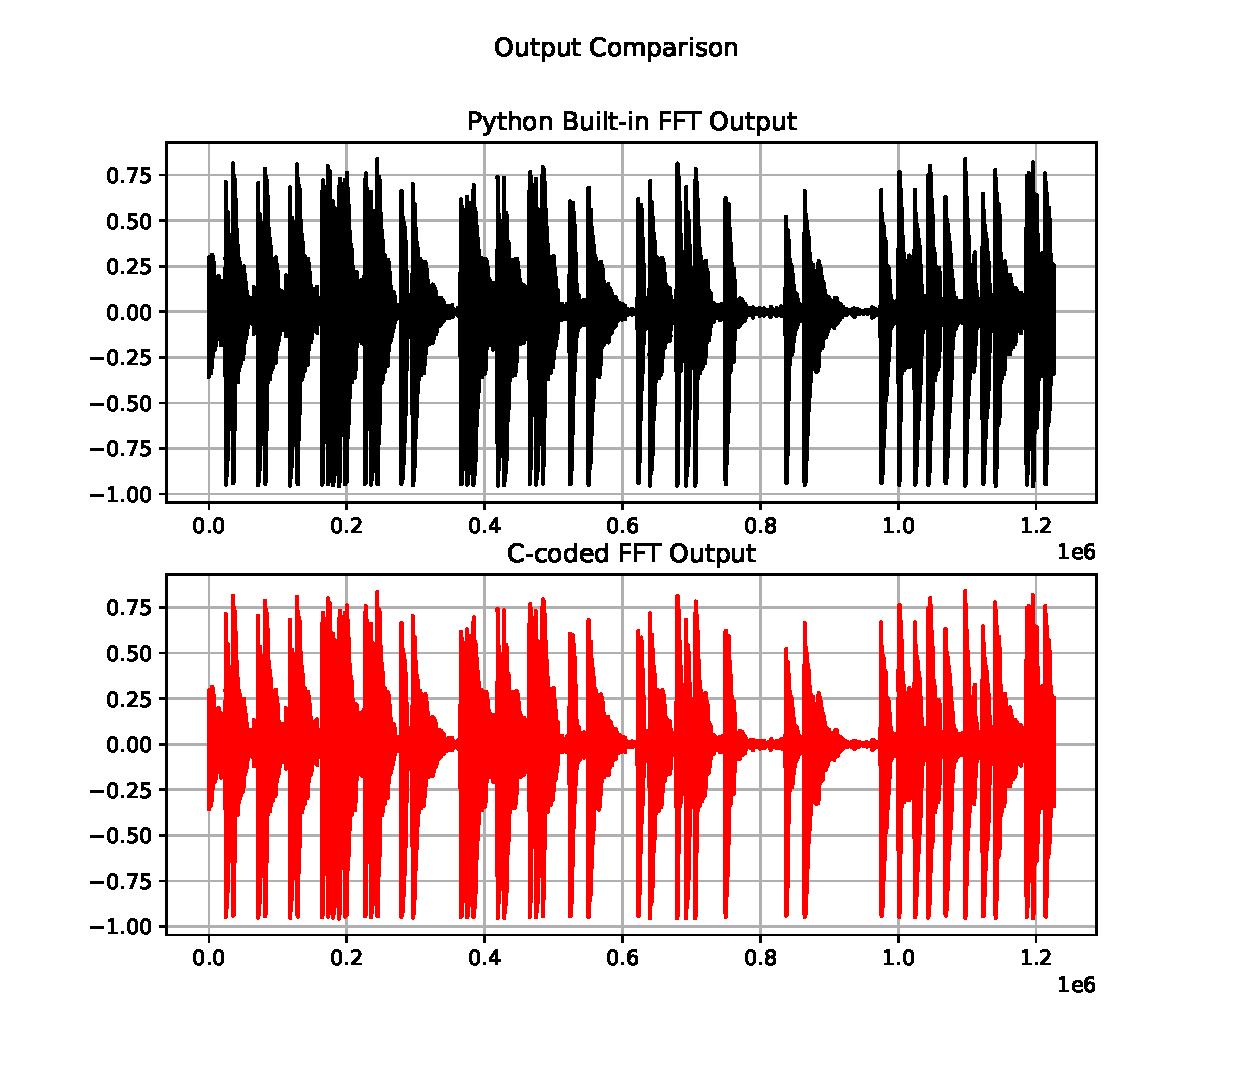
\includegraphics[width=1.2\columnwidth]{./figs/ee18btech11031.eps}
\caption{Time domain response}
\label{fig:Figure1}
\end{figure}

\end{document}
